\documentclass[12pt]{article}

% Invoke with
% pdflatex -jobname midterm-solutions "\def\showkey{}\documentclass[12pt]{article}

% Invoke with
% pdflatex -jobname midterm-solutions "\def\showkey{}\documentclass[12pt]{article}

% Invoke with
% pdflatex -jobname midterm-solutions "\def\showkey{}\documentclass[12pt]{article}

% Invoke with
% pdflatex -jobname midterm-solutions "\def\showkey{}\input{midterm.tex }"
% for solutions

\usepackage[T1]{fontenc}
\usepackage{fourier}
\usepackage[scaled=0.88]{luximono}
\usepackage{booktabs}
\usepackage{array}
\usepackage{tikz}
\usetikzlibrary{positioning,calc,automata}
\usepackage{listings}
\lstset{basicstyle=\ttfamily}
\usepackage{bbding}

\newif\ifkey

% \def\showkey{}

\ifdefined\showkey
  \keytrue
\else
  \keyfalse
\fi


\newcommand{\fillinbox}[1][X]{%
  \framebox[3pc]{\rule[-1.2pc]{0pt}{3pc}\ifkey \textcolor{red}{\Large #1} \fi}\hspace{5pt}}

\makeatletter
\newcommand\listofproblems{
  \problemline{\textbf{Problem}}{\textbf{Value}}{\textbf{Score}}{\textbf{Description}}
  \@starttoc{lop}
  \problemline{Total}{\arabic{total}}{}{}
}
\makeatother

\def\kleene#1#2#3#4{
\path [->] 
      (#1) edge node [above] {$\epsilon$} (#2)            
      (#3) edge node [above] {$\epsilon$} (#4)
      (#1) edge [bend right=50, looseness=1] node [below] {$\epsilon$} (#4)
      (#3) edge [bend right=85, looseness=1.2] node [above] {$\epsilon$} (#2)
;
}
\def\choice#1#2#3#4#5#6{
\path [->] 
      (#1) edge node [above left] {$\epsilon$} (#2)            
      (#1) edge node [below left] {$\epsilon$} (#3)
      (#4) edge node [above right] {$\epsilon$} (#6)            
      (#5) edge node [below right] {$\epsilon$} (#6)
;
}

\def\labelenumi{\alph{enumi})}

\def\problemline#1#2#3#4{\noindent\par\hspace{5pc}\hbox{\hbox to 3.5pc{\hfil#1\hfil}\hbox to 3.5pc{\hfil#2\hfil}\hbox to 6pc{\hfil#3\hfil}\hbox{#4}}\par\noindent\hspace{5pc}\rule{34pc}{0.5pt}}

\def\problemspec#1#2#3#4{\problemline{#1}{#2}{#3}{#4}
\addtocounter{total}{#2}}

\newcounter{problem}
\newenvironment{problem}[2]{
  \refstepcounter{problem}
  \par\noindent
  \arabic{problem}. (#1 pts.)
  \addtocontents{lop}{\protect\problemspec{\theproblem}{#1}{}{#2}}
}

\newcounter{total}

% Make ``.'' a mathrel symbol: improves spacing in lambda expressions
\mathcode`\.="313A

\tikzset{>=latex,double distance=2pt} % Nicer looking arrows

\usepackage[top=0.5in,bottom=1in,left=0.5in,right=0.5in]{geometry}

\begin{document}
\begin{titlepage}
\null\vspace{5pc}
\begin{center}
{\large
Columbia University \\
Computer Science Department \\
\medskip
COMS W4115 Programming Languages and Translators \\
Midterm \\
}
October 17, 2018\\
\end{center}

\vspace{3pc}

\hbox to \textwidth{Name: \ifkey \textcolor{red}{KEY KEY KEY KEY KEY} \fi \hrulefill}
\hbox to \textwidth{\hspace{2.5pc} First \quad Last (Family) \hfil Uni (e.g., se2007)}

\vspace{2pc}

\vspace{2pc}

\begin{itemize}
\item You may consult your own 8.5$''$ $\times$ 11$''$ double-sided sheet of
notes, but nothing else (e.g., no text, no other notes).
\item You may use a calculator, but probably don't need one.
\item Perform all work on the midterm itself.  Use the backs of the
pages if necessary.  \emph{Do not use scratch paper.}
\item Explain your answers.
\end{itemize}

\vspace{2pc}

\listofproblems

\end{titlepage}

\makeatletter
\def\@n#1{\node (#1) {#1};}
\def\@nn*#1{\node [double] (#1) {#1};}
\def\autonode{\@ifnextchar*{\@nn}{\@n}}
\makeatother

\tikzset{automaton/.style={every node/.style={circle,draw,minimum width=1.5pc},
  column sep=1pc,
  row sep=1pc,
  execute at begin cell=\autonode,
  execute at end cell=,
  execute at empty cell=}
}

\begin{problem}{15}{Thompson's Construction}
\textbf{Draw the NFA} for the
regular expression $a\ b^* (a\,|\,\epsilon\,|\,b)$ produced by \textbf{Thompson's construction}.

\vbox to 15pc{
\ifkey
\begin{tikzpicture}[color=red]
  \matrix [automaton] {
 & & & & & &6&7\\
 & & & & &5& & &{10}\\
 & & & & & &8&9\\
0&1&2&3&4& & & &    & *{13}\\
 & & & & & &{11}&{12}\\  
};
\kleene 1 2 3 4
\choice 4 5 {11} {10} {12} {13}
\choice 5 6 8 7 9 {10}
%\kleene {9} {10} {11} {12}
%\choice 0 1 6 5 8 9
\path [->] (0) edge node [above] {$a$} (1)
           (2) edge node [above] {$b$} (3)
           (6) edge node [above] {$a$} (7)
           (8) edge node [above] {$\epsilon$} (9)
           (11) edge node [above] {$b$} (12)
;
\end{tikzpicture}
\fi
\vfill
}

\end{problem}

\begin{problem}{25}{Subset Construction}
Consider the following NFA,
\begin{tikzpicture}[baseline=3pc]
\matrix [automaton] {
 &1&2&3&4&5 \\
0& & & & & & &{12}&*{13}\\
 &6&7&8&9&{10}&{11}\\
};
\kleene 2 3 4 5
\kleene 7 8 9 {10}
\choice 0 1 6 5 {11} {12}
\path [->] (1) edge node [above] {$a$} (2)
           (3) edge node [above] {$b$} (4)
           (6) edge node [above] {$b$} (7)
           (8) edge node [above] {$a$} (9)
           (10) edge node [above] {$\epsilon$} (11)
           (12) edge node [above] {$c$} (13)
;
\end{tikzpicture}

\begin{enumerate}
\item Write the \textbf{regular expression} that, were \textbf{Thompson's
  construction} applied, would produce this NFA.

\vbox to 3pc{
\vfill
\ifkey \textcolor{red}{$(a\,b^*\, |\ b\,a^*\,\epsilon)\, c$}\fi
\vfill
}

% http://hackingoff.com/compilers/regular-expression-to-nfa-dfa

\item Perform the \textbf{subset construction} algorithm.  Fill in the
  \textbf{table} and \textbf{draw} the corresponding DFA.  I've
  started the table for you.

{\renewcommand{\arraystretch}{1.2}\large
\ifkey\color{red}\fi
\begin{tabular}[b]{cp{14pc}ccc}
%\toprule
%\multicolumn{2}{@{}c@{}}{\textbf{Current State}} &
%\multicolumn{3}{@{}c@{}}{\textbf{Next State}} \\
%\cmidrule(r){1-2}
%\cmidrule(l){3-5}
\textbf{DFA} &
\multicolumn{1}{c}{\textbf{NFA}} &
$a$ & $b$ & $c$ \\
\midrule
A & \{ 0 1 6 \} & B & C & $-$ \\
\ifkey
B & \{ 2 3 5 12 \} & $-$ & D & E \\
C & \{ 7 8 10 11 12 \} & F & $-$ & E \\
D & \{ 3 4 5 12 \} & $-$ & D & E \\
E & \{ 13 \} & $-$ & $-$ & $-$ \\
F & \{ 8 9 10 11 12 \} & F & $-$ & E \\
\else
\\[10pc]
\fi
\end{tabular}
}
\ifkey
\begin{tikzpicture}[color=red]
\matrix [automaton] {
 &B&&D \\
A& &*E \\
 &C&&F \\
};
\path [->] (A) edge node [above left] {$a$} (B)
           (A) edge node [below left] {$b$} (C)
           (B) edge node [above] {$b$} (D)
           (B) edge node [below left] {$c$} (E)
           (C) edge node [below] {$a$} (F)
           (C) edge node [above left] {$c$} (E)
           (D) edge [loop above] node [above] {$b$} (D)
           (D) edge node [below right] {$c$} (E)
           (F) edge node [above right] {$c$} (E)
           (F) edge [loop below] node [below] {$a$} (G)
;
\end{tikzpicture}
\fi

\end{enumerate}

\end{problem}

\newpage

\begin{problem}{5}{DFAs, NFAs, and REs}

\begin{enumerate}

\item (3 pts)
Write the \textbf{simplest possible} regular expression that accepts
the same language as this DFA.

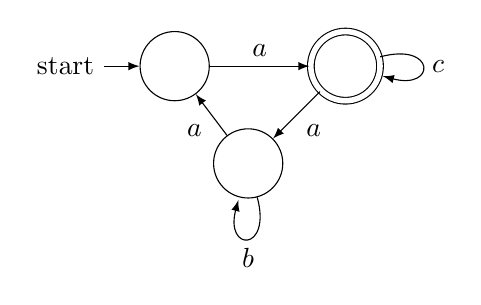
\begin{tikzpicture}[baseline=-2pc]
  \node [state,initial] (A) {};
  \node [state,right=3pc of A,accepting] (B) {};
  \node [state,below left=2pc of B] (C) {};
  \path [->] (A) edge node [above] {$a$} (B);
  \path [->] (B) edge [loop right] node [right] {$c$} ();
  \path [->] (C) edge [loop below] node [below] {$b$} ();
  \path [->] (B) edge node [below right] {$a$} (C);
  \path [->] (C) edge node [below left] {$a$} (A);
\end{tikzpicture}
\hfill
\ifkey{\color{red} $a(c|ab^*aa)^*$}\fi

\vspace{1pc}

\item (2 pts) Write the \textbf{simplest equivalent} regular expression for
  the following NFA.

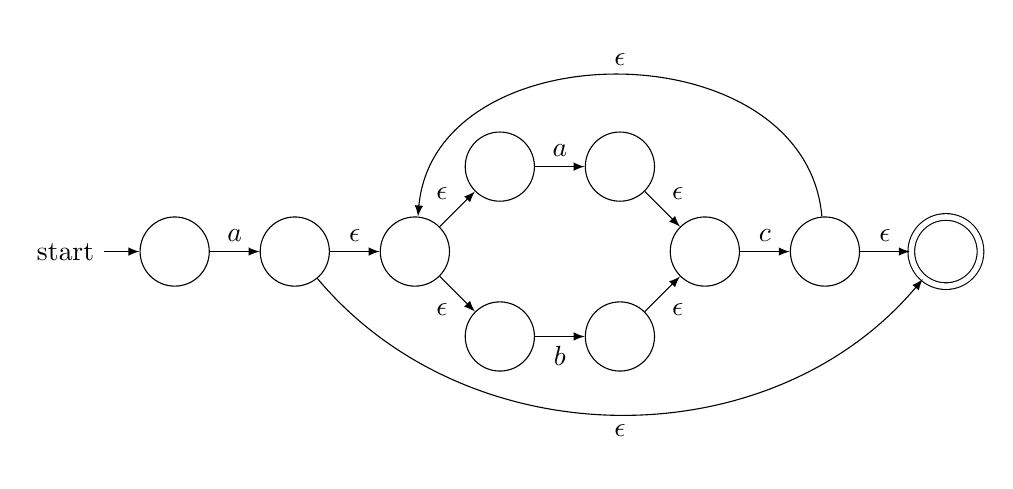
\begin{tikzpicture}[node distance=1.5pc,baseline=0pc]
    \node [state,initial] (00) {};
    \node [state,right=of 00] (0) {};
    \node [state,right=of 0] (1) {};
    \node [state,above right=of 1] (2) {};
    \node [state,right=of 2] (3) {};
    \node [state,below right=of 1] (4) {};
    \node [state,right=of 4] (5) {};
    \node [state,below right=of 3] (6) {};
    \node [state,right=of 6] (7) {};
    \node [state,right=of 7,accepting] (8) {};
    \path [->] (00) edge node [above] {$a$} (0)
               (2) edge node [above] {$a$} (3)
               (4) edge node [below] {$b$} (5)            
               (6) edge node [above] {$c$} (7)
    ;
    \choice 1 2 4 3 5 6
    \kleene 0 1 7 8
\end{tikzpicture}
\hfill
\ifkey{\color{red} $a\,((a\,|\,b)\,c)^*$}\fi

\end{enumerate}

\begin{problem}{10}{Grammars}
Write an \textbf{unambiguous grammar} that accepts the same language
as the grammar below, whose terminals are ``$\bigtriangleup$,''
``$\bigcirc$,'' and ``$a$.''  Make it so ``$\bigtriangleup$''
\textbf{associates left-to-right}, ``$\bigcirc$'' \textbf{associates
  right-to-left}, and ``$\bigtriangleup$'' is at a \textbf{higher
  level of precedence} than ``$\bigcirc$''.  E.g., so that
``$a\bigtriangleup a\bigtriangleup a \bigcirc a \bigcirc a$'' has a
unique rightmost derivation grouped like ``$(a\bigtriangleup
a)\bigtriangleup \big(a \bigcirc (a \bigcirc a)\big)$''

\[
\begin{array}{l}
E \rightarrow E\ \bigtriangleup\ E \\
E \rightarrow E\ \bigcirc\ E \\
E \rightarrow a
\end{array}
\]

\vbox to 8pc{
\ifkey{\color{red}
\[
\begin{array}{l}
E \rightarrow T\ \bigcirc\ E \\
E \rightarrow T \\
T \rightarrow T \ \bigtriangleup\ c \\
T \rightarrow a \\
\end{array}
\]
}\fi
\vfill
}
\end{problem}

\end{problem}

\newpage
\begin{problem}{25}{The SLR Parse Table}

Consider the grammar  \hspace{2pc}  \begin{tabular}[t]{>{\footnotesize}l>{$}l<{$}@{\ $\rightarrow$\ }>{$}l<{$}}
0: & X' & X \\
1: & X & b \\
2: & X & Y \\
3: & X & a X \\
4: & Y & b \\
\end{tabular}
\hspace{2pc}
\begin{minipage}[t]{16pc}
This generates strings of the form $a^*b$, e.g., $b$, $aaab$.  Here is
a derivation for the string $ab$ with the handles underlined:  $X'
\rightarrow \underline{X} \rightarrow \underline{a X} \rightarrow a
\underline{b}$.
\end{minipage}

\begin{enumerate}

\item (4 pts.) Show \textbf{two rightmost derivations} for $aab$
  and \textbf{underline the handles}.

\vbox to 4pc{
\ifkey\color{red}
$X' \rightarrow \underline{X} \rightarrow \underline{a X} \rightarrow a \underline{a X} \rightarrow a a \underline{b}$

$X' \rightarrow \underline{X} \rightarrow \underline{a X} \rightarrow a \underline{a X} \rightarrow a a \underline{Y}
\rightarrow a a \underline{b}$
\fi
\vfill
}

\item (4 pts.) Is this grammar ambiguous?  Why or why not?

\vbox to 3pc{

\ifkey
\color{red}Yes: there are two rightmost derivations for the same string.
\fi
\vfill
}

\item (4 pts.) Compute the following sets.  \textbf{Explain your reasoning.}

$\textsc{follow}(X) = \Bigg\{ \ifkey \textcolor{red} {\$} \fi \hspace{8pc} \Bigg\}$  \ifkey \quad \textcolor{red}{$X' \rightarrow X$ implies \$; $X \rightarrow a X$ gives nothing more} \fi

$\textsc{follow}(Y) = \Bigg\{ \ifkey \textcolor{red} {\$} \fi \hspace{8pc} \Bigg\}$ \ifkey \quad \textcolor{red}{$X \rightarrow Y$ implies \$; nothing further} \fi

\item (13 pts.)  Complete the \textbf{LR(0) automaton} and
  \textbf{SLR parse table} for this grammar. Mark all accepting states. \textbf{Indicate where
    the reduce/reduce error occurs.} 

\newcommand{\itemtab}[1]{
  \begin{tabular}{>{$}l<{$}@{\ $\rightarrow$\ }>{$}l<{$}} #1 
  \end{tabular}}

\vspace{2pc}

\ifkey
  \def\accepting{accepting}
\else
  \def\accepting{}
\fi


\begin{tikzpicture}[baseline=0pc]
\node [draw,minimum height=7pc,text width=8pc] (S0) {S0: 
  \itemtab{
    X' & \cdot X \\
    X & \cdot b \\
    X & \cdot Y \\
    X & \cdot a X \\
    Y & \cdot b}
  };

\node [draw,above right=of S0,minimum height=7pc,text width=8pc,\accepting] (S1) {
  S1: \ifkey\color{red}\itemtab{
    X & b \cdot \\
    Y & b \cdot}\fi
  };

\node [draw,right=of S0,minimum height=7pc, text width=8pc] (S2) {
  S2:
  \ifkey\color{red}\itemtab{
    X & a \cdot X \\
    X & \cdot b \\
    X & \cdot Y \\
    X & \cdot a X \\
    Y & \cdot b}\fi
  };

\node [draw,below=of S0,minimum height=7pc, text width=8pc, \accepting] (S3) {
  S3:
  \ifkey\color{red}\itemtab{
    X & Y \cdot}\fi
  };

\node [draw,below=of S2,minimum height=7pc, text width=8pc, \accepting] (S4) {
  S4:
  \ifkey\color{red}\itemtab{
    X & a X \cdot}\fi
  };


\node [draw,above=of S0,minimum height=7pc, text width=8pc, \accepting] (S5) {
  S5:
  \ifkey\color{red}\itemtab{
    X' & X \cdot}\fi
  };

\path [->] (S0) edge node [above left] {$b$} (S1)
                edge node [above] {$a$} (S2)
                edge node [right] {$Y$} (S3)
                edge node [right] {$X$} (S5);
\ifkey
\path [->,color=red]
           (S2) edge [out=5,in=-5,loop] node [right] {$a$} ()
                edge node [above] {$Y$} (S3)
                edge node [right] {$X$} (S4)
                edge node [right] {$b$} (S1);
\fi
\end{tikzpicture}
\hspace{3pc}
\setlength{\tabcolsep}{10pt}
\renewcommand{\arraystretch}{3}
\begin{tabular}{r|ccc|cc}
 & a & b & \$ & X & Y \\
\hline
0 & s2 & s1 & & 5 & 3 \\
1 & & &\ifkey\color{red} r1/4\fi & & \\
2 & \ifkey\color{red} s2\fi & \ifkey\color{red} s1\fi & & \ifkey\color{red} 4\fi & \ifkey\color{red} 3\fi\\
3 & & & \ifkey\color{red} r2\fi& & \\
4 & & & \ifkey\color{red} r3\fi& \\
5 & & & \ifkey\color{red} \Checkmark\fi& & \\
\end{tabular}

\vfill

\end{enumerate}

\end{problem}

\newpage

\if 0
http://jsmachines.sourceforge.net/machines/slr.html

E' -> E
E -> E * T
E -> T
T -> T + id
T -> id

1	0		id + id * id $	s3	
2	0 id 3		+ id * id $	r4
3	0 T		+ id * id $	2
4	0 T 2		+ id * id $	s5
5	0 T 2 + 5	id * id $	s7
6	0 T 2 + 5 	id 7	* id $	r3
7	0 T		* id $		2
8	0 T 2		* id $		r2
9	0 E		* id $		1
10	0 E 1		* id $		s4
11	0 E 1 * 4	id $		s3
12	0 E 1 * 4 id 3	$		r4
13	0 E 1 * 4 T	$		6
14	0 E 1 * 4 T 6	$		r1
15	0 E		$		1
16	0 E 1		$		acc

\fi

\begin{problem}{20}{Rightmost Derivations, Bottom-Up Parsing}

For the following grammar with terminals $\times$, $+$, and
\textbf{n} and non-terminals $T$ and $E$

\[
\begin{array}{rl}
1: & E \rightarrow E\ \times\ T \\
2: & E \rightarrow T \\
3: & T \rightarrow T\ +\ \textbf{n} \\
4: & T \rightarrow \textbf{n} \\
\end{array}
\]

\begin{enumerate}

\item (5pt) Give a \textbf{rightmost derivation} for ``\textbf{$n + n \times n$}'' and
  \textbf{underline the handles}.

\vbox to 8pc{
\ifkey{\color{red}
$
E
\rightarrow \underline{E \times T}
\rightarrow E \times \underline{n}
\rightarrow \underline{T} \times n
\rightarrow \underline{T + n} \times n
\rightarrow \underline{n} + n \times n
$
}
\fi
\vfill
}

\item (15 pts.) \textbf{Show the steps} a shift-reduce parser would
  take on such an input.  I've started the table for you.

\vspace{1pc}

\vbox to 20pc{
\begin{tabular}{@{\hspace{5pc}}rl@{\hspace{5pc}}l}
\toprule
\textbf{Stack} & \textbf{Input} & \textbf{Action} \\
\midrule
 & n + n $\times$ n \$ & Shift \\
\ifkey
\color{red}n &\color{red} + n $\times$ n \$ &\color{red} Reduce 4 \\
\color{red}T &\color{red} + n $\times$ n \$ &\color{red} Shift \\
\color{red}T + &\color{red} n $\times$ n \$ &\color{red} Shift \\
\color{red}T + n &\color{red} $\times$ n \$ &\color{red} Reduce 3 \\
\color{red}T     &\color{red} $\times$ n \$ &\color{red} Reduce 2 \\
\color{red}E     &\color{red} $\times$ n \$ &\color{red} Shift \\
\color{red}E $\times$     &\color{red} n \$ &\color{red} Shift \\
\color{red}E $\times$ n     &\color{red} \$ &\color{red} Reduce 4 \\
\color{red}E $\times$ T     &\color{red} \$ &\color{red} Reduce 1 \\
\color{red}E                &\color{red} \$ &\color{red} Accept \\
\fi
\end{tabular}
\vfill
}


\end{enumerate}

\end{problem}




\end{document}

% Local Variables:
% compile-command: "make midterm.pdf"
% End:
"
% for solutions

\usepackage[T1]{fontenc}
\usepackage{fourier}
\usepackage[scaled=0.88]{luximono}
\usepackage{booktabs}
\usepackage{array}
\usepackage{tikz}
\usetikzlibrary{positioning,calc,automata}
\usepackage{listings}
\lstset{basicstyle=\ttfamily}
\usepackage{bbding}

\newif\ifkey

% \def\showkey{}

\ifdefined\showkey
  \keytrue
\else
  \keyfalse
\fi


\newcommand{\fillinbox}[1][X]{%
  \framebox[3pc]{\rule[-1.2pc]{0pt}{3pc}\ifkey \textcolor{red}{\Large #1} \fi}\hspace{5pt}}

\makeatletter
\newcommand\listofproblems{
  \problemline{\textbf{Problem}}{\textbf{Value}}{\textbf{Score}}{\textbf{Description}}
  \@starttoc{lop}
  \problemline{Total}{\arabic{total}}{}{}
}
\makeatother

\def\kleene#1#2#3#4{
\path [->] 
      (#1) edge node [above] {$\epsilon$} (#2)            
      (#3) edge node [above] {$\epsilon$} (#4)
      (#1) edge [bend right=50, looseness=1] node [below] {$\epsilon$} (#4)
      (#3) edge [bend right=85, looseness=1.2] node [above] {$\epsilon$} (#2)
;
}
\def\choice#1#2#3#4#5#6{
\path [->] 
      (#1) edge node [above left] {$\epsilon$} (#2)            
      (#1) edge node [below left] {$\epsilon$} (#3)
      (#4) edge node [above right] {$\epsilon$} (#6)            
      (#5) edge node [below right] {$\epsilon$} (#6)
;
}

\def\labelenumi{\alph{enumi})}

\def\problemline#1#2#3#4{\noindent\par\hspace{5pc}\hbox{\hbox to 3.5pc{\hfil#1\hfil}\hbox to 3.5pc{\hfil#2\hfil}\hbox to 6pc{\hfil#3\hfil}\hbox{#4}}\par\noindent\hspace{5pc}\rule{34pc}{0.5pt}}

\def\problemspec#1#2#3#4{\problemline{#1}{#2}{#3}{#4}
\addtocounter{total}{#2}}

\newcounter{problem}
\newenvironment{problem}[2]{
  \refstepcounter{problem}
  \par\noindent
  \arabic{problem}. (#1 pts.)
  \addtocontents{lop}{\protect\problemspec{\theproblem}{#1}{}{#2}}
}

\newcounter{total}

% Make ``.'' a mathrel symbol: improves spacing in lambda expressions
\mathcode`\.="313A

\tikzset{>=latex,double distance=2pt} % Nicer looking arrows

\usepackage[top=0.5in,bottom=1in,left=0.5in,right=0.5in]{geometry}

\begin{document}
\begin{titlepage}
\null\vspace{5pc}
\begin{center}
{\large
Columbia University \\
Computer Science Department \\
\medskip
COMS W4115 Programming Languages and Translators \\
Midterm \\
}
October 17, 2018\\
\end{center}

\vspace{3pc}

\hbox to \textwidth{Name: \ifkey \textcolor{red}{KEY KEY KEY KEY KEY} \fi \hrulefill}
\hbox to \textwidth{\hspace{2.5pc} First \quad Last (Family) \hfil Uni (e.g., se2007)}

\vspace{2pc}

\vspace{2pc}

\begin{itemize}
\item You may consult your own 8.5$''$ $\times$ 11$''$ double-sided sheet of
notes, but nothing else (e.g., no text, no other notes).
\item You may use a calculator, but probably don't need one.
\item Perform all work on the midterm itself.  Use the backs of the
pages if necessary.  \emph{Do not use scratch paper.}
\item Explain your answers.
\end{itemize}

\vspace{2pc}

\listofproblems

\end{titlepage}

\makeatletter
\def\@n#1{\node (#1) {#1};}
\def\@nn*#1{\node [double] (#1) {#1};}
\def\autonode{\@ifnextchar*{\@nn}{\@n}}
\makeatother

\tikzset{automaton/.style={every node/.style={circle,draw,minimum width=1.5pc},
  column sep=1pc,
  row sep=1pc,
  execute at begin cell=\autonode,
  execute at end cell=,
  execute at empty cell=}
}

\begin{problem}{15}{Thompson's Construction}
\textbf{Draw the NFA} for the
regular expression $a\ b^* (a\,|\,\epsilon\,|\,b)$ produced by \textbf{Thompson's construction}.

\vbox to 15pc{
\ifkey
\begin{tikzpicture}[color=red]
  \matrix [automaton] {
 & & & & & &6&7\\
 & & & & &5& & &{10}\\
 & & & & & &8&9\\
0&1&2&3&4& & & &    & *{13}\\
 & & & & & &{11}&{12}\\  
};
\kleene 1 2 3 4
\choice 4 5 {11} {10} {12} {13}
\choice 5 6 8 7 9 {10}
%\kleene {9} {10} {11} {12}
%\choice 0 1 6 5 8 9
\path [->] (0) edge node [above] {$a$} (1)
           (2) edge node [above] {$b$} (3)
           (6) edge node [above] {$a$} (7)
           (8) edge node [above] {$\epsilon$} (9)
           (11) edge node [above] {$b$} (12)
;
\end{tikzpicture}
\fi
\vfill
}

\end{problem}

\begin{problem}{25}{Subset Construction}
Consider the following NFA,
\begin{tikzpicture}[baseline=3pc]
\matrix [automaton] {
 &1&2&3&4&5 \\
0& & & & & & &{12}&*{13}\\
 &6&7&8&9&{10}&{11}\\
};
\kleene 2 3 4 5
\kleene 7 8 9 {10}
\choice 0 1 6 5 {11} {12}
\path [->] (1) edge node [above] {$a$} (2)
           (3) edge node [above] {$b$} (4)
           (6) edge node [above] {$b$} (7)
           (8) edge node [above] {$a$} (9)
           (10) edge node [above] {$\epsilon$} (11)
           (12) edge node [above] {$c$} (13)
;
\end{tikzpicture}

\begin{enumerate}
\item Write the \textbf{regular expression} that, were \textbf{Thompson's
  construction} applied, would produce this NFA.

\vbox to 3pc{
\vfill
\ifkey \textcolor{red}{$(a\,b^*\, |\ b\,a^*\,\epsilon)\, c$}\fi
\vfill
}

% http://hackingoff.com/compilers/regular-expression-to-nfa-dfa

\item Perform the \textbf{subset construction} algorithm.  Fill in the
  \textbf{table} and \textbf{draw} the corresponding DFA.  I've
  started the table for you.

{\renewcommand{\arraystretch}{1.2}\large
\ifkey\color{red}\fi
\begin{tabular}[b]{cp{14pc}ccc}
%\toprule
%\multicolumn{2}{@{}c@{}}{\textbf{Current State}} &
%\multicolumn{3}{@{}c@{}}{\textbf{Next State}} \\
%\cmidrule(r){1-2}
%\cmidrule(l){3-5}
\textbf{DFA} &
\multicolumn{1}{c}{\textbf{NFA}} &
$a$ & $b$ & $c$ \\
\midrule
A & \{ 0 1 6 \} & B & C & $-$ \\
\ifkey
B & \{ 2 3 5 12 \} & $-$ & D & E \\
C & \{ 7 8 10 11 12 \} & F & $-$ & E \\
D & \{ 3 4 5 12 \} & $-$ & D & E \\
E & \{ 13 \} & $-$ & $-$ & $-$ \\
F & \{ 8 9 10 11 12 \} & F & $-$ & E \\
\else
\\[10pc]
\fi
\end{tabular}
}
\ifkey
\begin{tikzpicture}[color=red]
\matrix [automaton] {
 &B&&D \\
A& &*E \\
 &C&&F \\
};
\path [->] (A) edge node [above left] {$a$} (B)
           (A) edge node [below left] {$b$} (C)
           (B) edge node [above] {$b$} (D)
           (B) edge node [below left] {$c$} (E)
           (C) edge node [below] {$a$} (F)
           (C) edge node [above left] {$c$} (E)
           (D) edge [loop above] node [above] {$b$} (D)
           (D) edge node [below right] {$c$} (E)
           (F) edge node [above right] {$c$} (E)
           (F) edge [loop below] node [below] {$a$} (G)
;
\end{tikzpicture}
\fi

\end{enumerate}

\end{problem}

\newpage

\begin{problem}{5}{DFAs, NFAs, and REs}

\begin{enumerate}

\item (3 pts)
Write the \textbf{simplest possible} regular expression that accepts
the same language as this DFA.

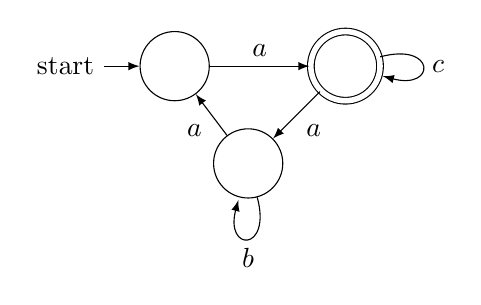
\begin{tikzpicture}[baseline=-2pc]
  \node [state,initial] (A) {};
  \node [state,right=3pc of A,accepting] (B) {};
  \node [state,below left=2pc of B] (C) {};
  \path [->] (A) edge node [above] {$a$} (B);
  \path [->] (B) edge [loop right] node [right] {$c$} ();
  \path [->] (C) edge [loop below] node [below] {$b$} ();
  \path [->] (B) edge node [below right] {$a$} (C);
  \path [->] (C) edge node [below left] {$a$} (A);
\end{tikzpicture}
\hfill
\ifkey{\color{red} $a(c|ab^*aa)^*$}\fi

\vspace{1pc}

\item (2 pts) Write the \textbf{simplest equivalent} regular expression for
  the following NFA.

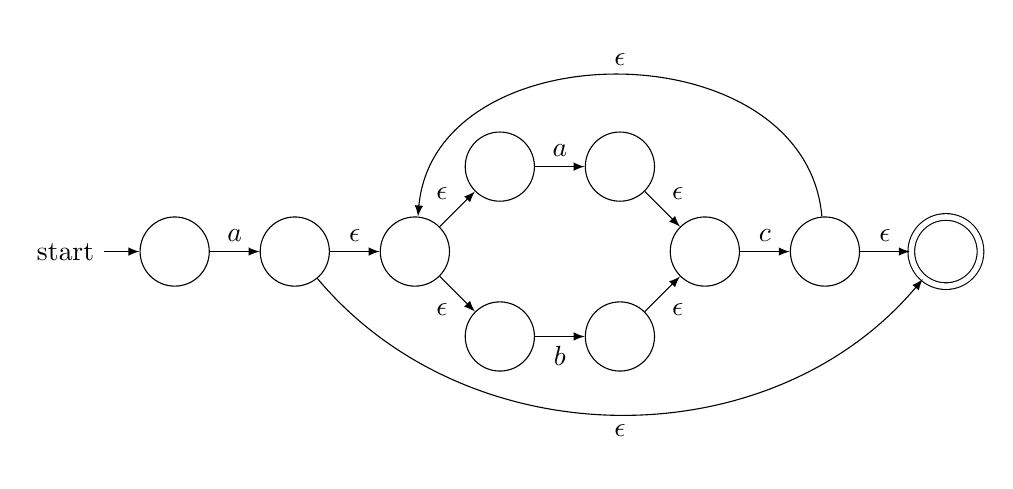
\begin{tikzpicture}[node distance=1.5pc,baseline=0pc]
    \node [state,initial] (00) {};
    \node [state,right=of 00] (0) {};
    \node [state,right=of 0] (1) {};
    \node [state,above right=of 1] (2) {};
    \node [state,right=of 2] (3) {};
    \node [state,below right=of 1] (4) {};
    \node [state,right=of 4] (5) {};
    \node [state,below right=of 3] (6) {};
    \node [state,right=of 6] (7) {};
    \node [state,right=of 7,accepting] (8) {};
    \path [->] (00) edge node [above] {$a$} (0)
               (2) edge node [above] {$a$} (3)
               (4) edge node [below] {$b$} (5)            
               (6) edge node [above] {$c$} (7)
    ;
    \choice 1 2 4 3 5 6
    \kleene 0 1 7 8
\end{tikzpicture}
\hfill
\ifkey{\color{red} $a\,((a\,|\,b)\,c)^*$}\fi

\end{enumerate}

\begin{problem}{10}{Grammars}
Write an \textbf{unambiguous grammar} that accepts the same language
as the grammar below, whose terminals are ``$\bigtriangleup$,''
``$\bigcirc$,'' and ``$a$.''  Make it so ``$\bigtriangleup$''
\textbf{associates left-to-right}, ``$\bigcirc$'' \textbf{associates
  right-to-left}, and ``$\bigtriangleup$'' is at a \textbf{higher
  level of precedence} than ``$\bigcirc$''.  E.g., so that
``$a\bigtriangleup a\bigtriangleup a \bigcirc a \bigcirc a$'' has a
unique rightmost derivation grouped like ``$(a\bigtriangleup
a)\bigtriangleup \big(a \bigcirc (a \bigcirc a)\big)$''

\[
\begin{array}{l}
E \rightarrow E\ \bigtriangleup\ E \\
E \rightarrow E\ \bigcirc\ E \\
E \rightarrow a
\end{array}
\]

\vbox to 8pc{
\ifkey{\color{red}
\[
\begin{array}{l}
E \rightarrow T\ \bigcirc\ E \\
E \rightarrow T \\
T \rightarrow T \ \bigtriangleup\ c \\
T \rightarrow a \\
\end{array}
\]
}\fi
\vfill
}
\end{problem}

\end{problem}

\newpage
\begin{problem}{25}{The SLR Parse Table}

Consider the grammar  \hspace{2pc}  \begin{tabular}[t]{>{\footnotesize}l>{$}l<{$}@{\ $\rightarrow$\ }>{$}l<{$}}
0: & X' & X \\
1: & X & b \\
2: & X & Y \\
3: & X & a X \\
4: & Y & b \\
\end{tabular}
\hspace{2pc}
\begin{minipage}[t]{16pc}
This generates strings of the form $a^*b$, e.g., $b$, $aaab$.  Here is
a derivation for the string $ab$ with the handles underlined:  $X'
\rightarrow \underline{X} \rightarrow \underline{a X} \rightarrow a
\underline{b}$.
\end{minipage}

\begin{enumerate}

\item (4 pts.) Show \textbf{two rightmost derivations} for $aab$
  and \textbf{underline the handles}.

\vbox to 4pc{
\ifkey\color{red}
$X' \rightarrow \underline{X} \rightarrow \underline{a X} \rightarrow a \underline{a X} \rightarrow a a \underline{b}$

$X' \rightarrow \underline{X} \rightarrow \underline{a X} \rightarrow a \underline{a X} \rightarrow a a \underline{Y}
\rightarrow a a \underline{b}$
\fi
\vfill
}

\item (4 pts.) Is this grammar ambiguous?  Why or why not?

\vbox to 3pc{

\ifkey
\color{red}Yes: there are two rightmost derivations for the same string.
\fi
\vfill
}

\item (4 pts.) Compute the following sets.  \textbf{Explain your reasoning.}

$\textsc{follow}(X) = \Bigg\{ \ifkey \textcolor{red} {\$} \fi \hspace{8pc} \Bigg\}$  \ifkey \quad \textcolor{red}{$X' \rightarrow X$ implies \$; $X \rightarrow a X$ gives nothing more} \fi

$\textsc{follow}(Y) = \Bigg\{ \ifkey \textcolor{red} {\$} \fi \hspace{8pc} \Bigg\}$ \ifkey \quad \textcolor{red}{$X \rightarrow Y$ implies \$; nothing further} \fi

\item (13 pts.)  Complete the \textbf{LR(0) automaton} and
  \textbf{SLR parse table} for this grammar. Mark all accepting states. \textbf{Indicate where
    the reduce/reduce error occurs.} 

\newcommand{\itemtab}[1]{
  \begin{tabular}{>{$}l<{$}@{\ $\rightarrow$\ }>{$}l<{$}} #1 
  \end{tabular}}

\vspace{2pc}

\ifkey
  \def\accepting{accepting}
\else
  \def\accepting{}
\fi


\begin{tikzpicture}[baseline=0pc]
\node [draw,minimum height=7pc,text width=8pc] (S0) {S0: 
  \itemtab{
    X' & \cdot X \\
    X & \cdot b \\
    X & \cdot Y \\
    X & \cdot a X \\
    Y & \cdot b}
  };

\node [draw,above right=of S0,minimum height=7pc,text width=8pc,\accepting] (S1) {
  S1: \ifkey\color{red}\itemtab{
    X & b \cdot \\
    Y & b \cdot}\fi
  };

\node [draw,right=of S0,minimum height=7pc, text width=8pc] (S2) {
  S2:
  \ifkey\color{red}\itemtab{
    X & a \cdot X \\
    X & \cdot b \\
    X & \cdot Y \\
    X & \cdot a X \\
    Y & \cdot b}\fi
  };

\node [draw,below=of S0,minimum height=7pc, text width=8pc, \accepting] (S3) {
  S3:
  \ifkey\color{red}\itemtab{
    X & Y \cdot}\fi
  };

\node [draw,below=of S2,minimum height=7pc, text width=8pc, \accepting] (S4) {
  S4:
  \ifkey\color{red}\itemtab{
    X & a X \cdot}\fi
  };


\node [draw,above=of S0,minimum height=7pc, text width=8pc, \accepting] (S5) {
  S5:
  \ifkey\color{red}\itemtab{
    X' & X \cdot}\fi
  };

\path [->] (S0) edge node [above left] {$b$} (S1)
                edge node [above] {$a$} (S2)
                edge node [right] {$Y$} (S3)
                edge node [right] {$X$} (S5);
\ifkey
\path [->,color=red]
           (S2) edge [out=5,in=-5,loop] node [right] {$a$} ()
                edge node [above] {$Y$} (S3)
                edge node [right] {$X$} (S4)
                edge node [right] {$b$} (S1);
\fi
\end{tikzpicture}
\hspace{3pc}
\setlength{\tabcolsep}{10pt}
\renewcommand{\arraystretch}{3}
\begin{tabular}{r|ccc|cc}
 & a & b & \$ & X & Y \\
\hline
0 & s2 & s1 & & 5 & 3 \\
1 & & &\ifkey\color{red} r1/4\fi & & \\
2 & \ifkey\color{red} s2\fi & \ifkey\color{red} s1\fi & & \ifkey\color{red} 4\fi & \ifkey\color{red} 3\fi\\
3 & & & \ifkey\color{red} r2\fi& & \\
4 & & & \ifkey\color{red} r3\fi& \\
5 & & & \ifkey\color{red} \Checkmark\fi& & \\
\end{tabular}

\vfill

\end{enumerate}

\end{problem}

\newpage

\if 0
http://jsmachines.sourceforge.net/machines/slr.html

E' -> E
E -> E * T
E -> T
T -> T + id
T -> id

1	0		id + id * id $	s3	
2	0 id 3		+ id * id $	r4
3	0 T		+ id * id $	2
4	0 T 2		+ id * id $	s5
5	0 T 2 + 5	id * id $	s7
6	0 T 2 + 5 	id 7	* id $	r3
7	0 T		* id $		2
8	0 T 2		* id $		r2
9	0 E		* id $		1
10	0 E 1		* id $		s4
11	0 E 1 * 4	id $		s3
12	0 E 1 * 4 id 3	$		r4
13	0 E 1 * 4 T	$		6
14	0 E 1 * 4 T 6	$		r1
15	0 E		$		1
16	0 E 1		$		acc

\fi

\begin{problem}{20}{Rightmost Derivations, Bottom-Up Parsing}

For the following grammar with terminals $\times$, $+$, and
\textbf{n} and non-terminals $T$ and $E$

\[
\begin{array}{rl}
1: & E \rightarrow E\ \times\ T \\
2: & E \rightarrow T \\
3: & T \rightarrow T\ +\ \textbf{n} \\
4: & T \rightarrow \textbf{n} \\
\end{array}
\]

\begin{enumerate}

\item (5pt) Give a \textbf{rightmost derivation} for ``\textbf{$n + n \times n$}'' and
  \textbf{underline the handles}.

\vbox to 8pc{
\ifkey{\color{red}
$
E
\rightarrow \underline{E \times T}
\rightarrow E \times \underline{n}
\rightarrow \underline{T} \times n
\rightarrow \underline{T + n} \times n
\rightarrow \underline{n} + n \times n
$
}
\fi
\vfill
}

\item (15 pts.) \textbf{Show the steps} a shift-reduce parser would
  take on such an input.  I've started the table for you.

\vspace{1pc}

\vbox to 20pc{
\begin{tabular}{@{\hspace{5pc}}rl@{\hspace{5pc}}l}
\toprule
\textbf{Stack} & \textbf{Input} & \textbf{Action} \\
\midrule
 & n + n $\times$ n \$ & Shift \\
\ifkey
\color{red}n &\color{red} + n $\times$ n \$ &\color{red} Reduce 4 \\
\color{red}T &\color{red} + n $\times$ n \$ &\color{red} Shift \\
\color{red}T + &\color{red} n $\times$ n \$ &\color{red} Shift \\
\color{red}T + n &\color{red} $\times$ n \$ &\color{red} Reduce 3 \\
\color{red}T     &\color{red} $\times$ n \$ &\color{red} Reduce 2 \\
\color{red}E     &\color{red} $\times$ n \$ &\color{red} Shift \\
\color{red}E $\times$     &\color{red} n \$ &\color{red} Shift \\
\color{red}E $\times$ n     &\color{red} \$ &\color{red} Reduce 4 \\
\color{red}E $\times$ T     &\color{red} \$ &\color{red} Reduce 1 \\
\color{red}E                &\color{red} \$ &\color{red} Accept \\
\fi
\end{tabular}
\vfill
}


\end{enumerate}

\end{problem}




\end{document}

% Local Variables:
% compile-command: "make midterm.pdf"
% End:
"
% for solutions

\usepackage[T1]{fontenc}
\usepackage{fourier}
\usepackage[scaled=0.88]{luximono}
\usepackage{booktabs}
\usepackage{array}
\usepackage{tikz}
\usetikzlibrary{positioning,calc,automata}
\usepackage{listings}
\lstset{basicstyle=\ttfamily}
\usepackage{bbding}

\newif\ifkey

% \def\showkey{}

\ifdefined\showkey
  \keytrue
\else
  \keyfalse
\fi


\newcommand{\fillinbox}[1][X]{%
  \framebox[3pc]{\rule[-1.2pc]{0pt}{3pc}\ifkey \textcolor{red}{\Large #1} \fi}\hspace{5pt}}

\makeatletter
\newcommand\listofproblems{
  \problemline{\textbf{Problem}}{\textbf{Value}}{\textbf{Score}}{\textbf{Description}}
  \@starttoc{lop}
  \problemline{Total}{\arabic{total}}{}{}
}
\makeatother

\def\kleene#1#2#3#4{
\path [->] 
      (#1) edge node [above] {$\epsilon$} (#2)            
      (#3) edge node [above] {$\epsilon$} (#4)
      (#1) edge [bend right=50, looseness=1] node [below] {$\epsilon$} (#4)
      (#3) edge [bend right=85, looseness=1.2] node [above] {$\epsilon$} (#2)
;
}
\def\choice#1#2#3#4#5#6{
\path [->] 
      (#1) edge node [above left] {$\epsilon$} (#2)            
      (#1) edge node [below left] {$\epsilon$} (#3)
      (#4) edge node [above right] {$\epsilon$} (#6)            
      (#5) edge node [below right] {$\epsilon$} (#6)
;
}

\def\labelenumi{\alph{enumi})}

\def\problemline#1#2#3#4{\noindent\par\hspace{5pc}\hbox{\hbox to 3.5pc{\hfil#1\hfil}\hbox to 3.5pc{\hfil#2\hfil}\hbox to 6pc{\hfil#3\hfil}\hbox{#4}}\par\noindent\hspace{5pc}\rule{34pc}{0.5pt}}

\def\problemspec#1#2#3#4{\problemline{#1}{#2}{#3}{#4}
\addtocounter{total}{#2}}

\newcounter{problem}
\newenvironment{problem}[2]{
  \refstepcounter{problem}
  \par\noindent
  \arabic{problem}. (#1 pts.)
  \addtocontents{lop}{\protect\problemspec{\theproblem}{#1}{}{#2}}
}

\newcounter{total}

% Make ``.'' a mathrel symbol: improves spacing in lambda expressions
\mathcode`\.="313A

\tikzset{>=latex,double distance=2pt} % Nicer looking arrows

\usepackage[top=0.5in,bottom=1in,left=0.5in,right=0.5in]{geometry}

\begin{document}
\begin{titlepage}
\null\vspace{5pc}
\begin{center}
{\large
Columbia University \\
Computer Science Department \\
\medskip
COMS W4115 Programming Languages and Translators \\
Midterm \\
}
October 17, 2018\\
\end{center}

\vspace{3pc}

\hbox to \textwidth{Name: \ifkey \textcolor{red}{KEY KEY KEY KEY KEY} \fi \hrulefill}
\hbox to \textwidth{\hspace{2.5pc} First \quad Last (Family) \hfil Uni (e.g., se2007)}

\vspace{2pc}

\vspace{2pc}

\begin{itemize}
\item You may consult your own 8.5$''$ $\times$ 11$''$ double-sided sheet of
notes, but nothing else (e.g., no text, no other notes).
\item You may use a calculator, but probably don't need one.
\item Perform all work on the midterm itself.  Use the backs of the
pages if necessary.  \emph{Do not use scratch paper.}
\item Explain your answers.
\end{itemize}

\vspace{2pc}

\listofproblems

\end{titlepage}

\makeatletter
\def\@n#1{\node (#1) {#1};}
\def\@nn*#1{\node [double] (#1) {#1};}
\def\autonode{\@ifnextchar*{\@nn}{\@n}}
\makeatother

\tikzset{automaton/.style={every node/.style={circle,draw,minimum width=1.5pc},
  column sep=1pc,
  row sep=1pc,
  execute at begin cell=\autonode,
  execute at end cell=,
  execute at empty cell=}
}

\begin{problem}{15}{Thompson's Construction}
\textbf{Draw the NFA} for the
regular expression $a\ b^* (a\,|\,\epsilon\,|\,b)$ produced by \textbf{Thompson's construction}.

\vbox to 15pc{
\ifkey
\begin{tikzpicture}[color=red]
  \matrix [automaton] {
 & & & & & &6&7\\
 & & & & &5& & &{10}\\
 & & & & & &8&9\\
0&1&2&3&4& & & &    & *{13}\\
 & & & & & &{11}&{12}\\  
};
\kleene 1 2 3 4
\choice 4 5 {11} {10} {12} {13}
\choice 5 6 8 7 9 {10}
%\kleene {9} {10} {11} {12}
%\choice 0 1 6 5 8 9
\path [->] (0) edge node [above] {$a$} (1)
           (2) edge node [above] {$b$} (3)
           (6) edge node [above] {$a$} (7)
           (8) edge node [above] {$\epsilon$} (9)
           (11) edge node [above] {$b$} (12)
;
\end{tikzpicture}
\fi
\vfill
}

\end{problem}

\begin{problem}{25}{Subset Construction}
Consider the following NFA,
\begin{tikzpicture}[baseline=3pc]
\matrix [automaton] {
 &1&2&3&4&5 \\
0& & & & & & &{12}&*{13}\\
 &6&7&8&9&{10}&{11}\\
};
\kleene 2 3 4 5
\kleene 7 8 9 {10}
\choice 0 1 6 5 {11} {12}
\path [->] (1) edge node [above] {$a$} (2)
           (3) edge node [above] {$b$} (4)
           (6) edge node [above] {$b$} (7)
           (8) edge node [above] {$a$} (9)
           (10) edge node [above] {$\epsilon$} (11)
           (12) edge node [above] {$c$} (13)
;
\end{tikzpicture}

\begin{enumerate}
\item Write the \textbf{regular expression} that, were \textbf{Thompson's
  construction} applied, would produce this NFA.

\vbox to 3pc{
\vfill
\ifkey \textcolor{red}{$(a\,b^*\, |\ b\,a^*\,\epsilon)\, c$}\fi
\vfill
}

% http://hackingoff.com/compilers/regular-expression-to-nfa-dfa

\item Perform the \textbf{subset construction} algorithm.  Fill in the
  \textbf{table} and \textbf{draw} the corresponding DFA.  I've
  started the table for you.

{\renewcommand{\arraystretch}{1.2}\large
\ifkey\color{red}\fi
\begin{tabular}[b]{cp{14pc}ccc}
%\toprule
%\multicolumn{2}{@{}c@{}}{\textbf{Current State}} &
%\multicolumn{3}{@{}c@{}}{\textbf{Next State}} \\
%\cmidrule(r){1-2}
%\cmidrule(l){3-5}
\textbf{DFA} &
\multicolumn{1}{c}{\textbf{NFA}} &
$a$ & $b$ & $c$ \\
\midrule
A & \{ 0 1 6 \} & B & C & $-$ \\
\ifkey
B & \{ 2 3 5 12 \} & $-$ & D & E \\
C & \{ 7 8 10 11 12 \} & F & $-$ & E \\
D & \{ 3 4 5 12 \} & $-$ & D & E \\
E & \{ 13 \} & $-$ & $-$ & $-$ \\
F & \{ 8 9 10 11 12 \} & F & $-$ & E \\
\else
\\[10pc]
\fi
\end{tabular}
}
\ifkey
\begin{tikzpicture}[color=red]
\matrix [automaton] {
 &B&&D \\
A& &*E \\
 &C&&F \\
};
\path [->] (A) edge node [above left] {$a$} (B)
           (A) edge node [below left] {$b$} (C)
           (B) edge node [above] {$b$} (D)
           (B) edge node [below left] {$c$} (E)
           (C) edge node [below] {$a$} (F)
           (C) edge node [above left] {$c$} (E)
           (D) edge [loop above] node [above] {$b$} (D)
           (D) edge node [below right] {$c$} (E)
           (F) edge node [above right] {$c$} (E)
           (F) edge [loop below] node [below] {$a$} (G)
;
\end{tikzpicture}
\fi

\end{enumerate}

\end{problem}

\newpage

\begin{problem}{5}{DFAs, NFAs, and REs}

\begin{enumerate}

\item (3 pts)
Write the \textbf{simplest possible} regular expression that accepts
the same language as this DFA.

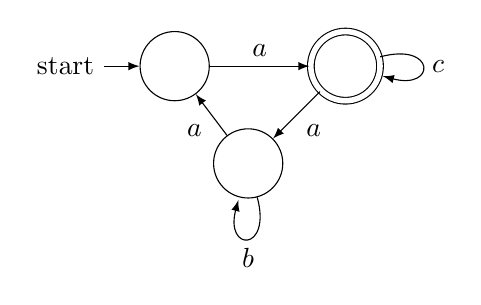
\begin{tikzpicture}[baseline=-2pc]
  \node [state,initial] (A) {};
  \node [state,right=3pc of A,accepting] (B) {};
  \node [state,below left=2pc of B] (C) {};
  \path [->] (A) edge node [above] {$a$} (B);
  \path [->] (B) edge [loop right] node [right] {$c$} ();
  \path [->] (C) edge [loop below] node [below] {$b$} ();
  \path [->] (B) edge node [below right] {$a$} (C);
  \path [->] (C) edge node [below left] {$a$} (A);
\end{tikzpicture}
\hfill
\ifkey{\color{red} $a(c|ab^*aa)^*$}\fi

\vspace{1pc}

\item (2 pts) Write the \textbf{simplest equivalent} regular expression for
  the following NFA.

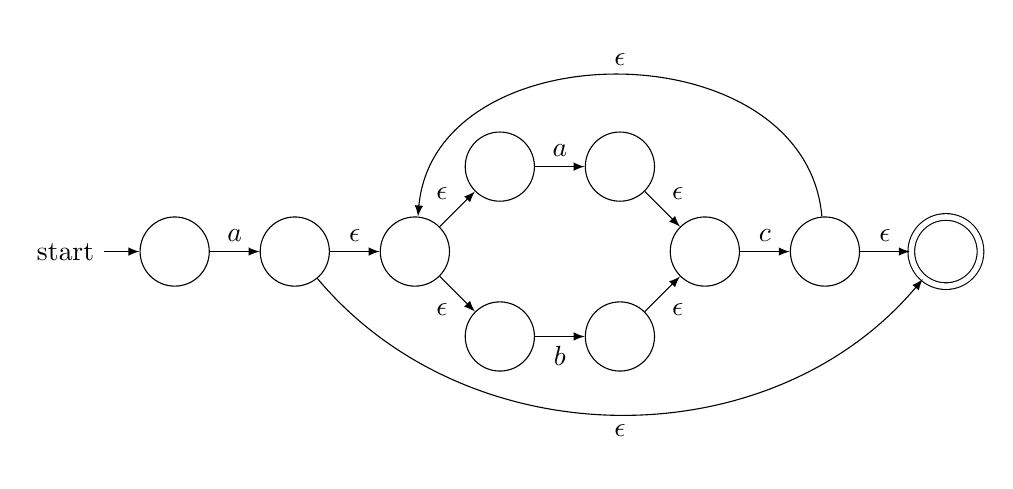
\begin{tikzpicture}[node distance=1.5pc,baseline=0pc]
    \node [state,initial] (00) {};
    \node [state,right=of 00] (0) {};
    \node [state,right=of 0] (1) {};
    \node [state,above right=of 1] (2) {};
    \node [state,right=of 2] (3) {};
    \node [state,below right=of 1] (4) {};
    \node [state,right=of 4] (5) {};
    \node [state,below right=of 3] (6) {};
    \node [state,right=of 6] (7) {};
    \node [state,right=of 7,accepting] (8) {};
    \path [->] (00) edge node [above] {$a$} (0)
               (2) edge node [above] {$a$} (3)
               (4) edge node [below] {$b$} (5)            
               (6) edge node [above] {$c$} (7)
    ;
    \choice 1 2 4 3 5 6
    \kleene 0 1 7 8
\end{tikzpicture}
\hfill
\ifkey{\color{red} $a\,((a\,|\,b)\,c)^*$}\fi

\end{enumerate}

\begin{problem}{10}{Grammars}
Write an \textbf{unambiguous grammar} that accepts the same language
as the grammar below, whose terminals are ``$\bigtriangleup$,''
``$\bigcirc$,'' and ``$a$.''  Make it so ``$\bigtriangleup$''
\textbf{associates left-to-right}, ``$\bigcirc$'' \textbf{associates
  right-to-left}, and ``$\bigtriangleup$'' is at a \textbf{higher
  level of precedence} than ``$\bigcirc$''.  E.g., so that
``$a\bigtriangleup a\bigtriangleup a \bigcirc a \bigcirc a$'' has a
unique rightmost derivation grouped like ``$(a\bigtriangleup
a)\bigtriangleup \big(a \bigcirc (a \bigcirc a)\big)$''

\[
\begin{array}{l}
E \rightarrow E\ \bigtriangleup\ E \\
E \rightarrow E\ \bigcirc\ E \\
E \rightarrow a
\end{array}
\]

\vbox to 8pc{
\ifkey{\color{red}
\[
\begin{array}{l}
E \rightarrow T\ \bigcirc\ E \\
E \rightarrow T \\
T \rightarrow T \ \bigtriangleup\ c \\
T \rightarrow a \\
\end{array}
\]
}\fi
\vfill
}
\end{problem}

\end{problem}

\newpage
\begin{problem}{25}{The SLR Parse Table}

Consider the grammar  \hspace{2pc}  \begin{tabular}[t]{>{\footnotesize}l>{$}l<{$}@{\ $\rightarrow$\ }>{$}l<{$}}
0: & X' & X \\
1: & X & b \\
2: & X & Y \\
3: & X & a X \\
4: & Y & b \\
\end{tabular}
\hspace{2pc}
\begin{minipage}[t]{16pc}
This generates strings of the form $a^*b$, e.g., $b$, $aaab$.  Here is
a derivation for the string $ab$ with the handles underlined:  $X'
\rightarrow \underline{X} \rightarrow \underline{a X} \rightarrow a
\underline{b}$.
\end{minipage}

\begin{enumerate}

\item (4 pts.) Show \textbf{two rightmost derivations} for $aab$
  and \textbf{underline the handles}.

\vbox to 4pc{
\ifkey\color{red}
$X' \rightarrow \underline{X} \rightarrow \underline{a X} \rightarrow a \underline{a X} \rightarrow a a \underline{b}$

$X' \rightarrow \underline{X} \rightarrow \underline{a X} \rightarrow a \underline{a X} \rightarrow a a \underline{Y}
\rightarrow a a \underline{b}$
\fi
\vfill
}

\item (4 pts.) Is this grammar ambiguous?  Why or why not?

\vbox to 3pc{

\ifkey
\color{red}Yes: there are two rightmost derivations for the same string.
\fi
\vfill
}

\item (4 pts.) Compute the following sets.  \textbf{Explain your reasoning.}

$\textsc{follow}(X) = \Bigg\{ \ifkey \textcolor{red} {\$} \fi \hspace{8pc} \Bigg\}$  \ifkey \quad \textcolor{red}{$X' \rightarrow X$ implies \$; $X \rightarrow a X$ gives nothing more} \fi

$\textsc{follow}(Y) = \Bigg\{ \ifkey \textcolor{red} {\$} \fi \hspace{8pc} \Bigg\}$ \ifkey \quad \textcolor{red}{$X \rightarrow Y$ implies \$; nothing further} \fi

\item (13 pts.)  Complete the \textbf{LR(0) automaton} and
  \textbf{SLR parse table} for this grammar. Mark all accepting states. \textbf{Indicate where
    the reduce/reduce error occurs.} 

\newcommand{\itemtab}[1]{
  \begin{tabular}{>{$}l<{$}@{\ $\rightarrow$\ }>{$}l<{$}} #1 
  \end{tabular}}

\vspace{2pc}

\ifkey
  \def\accepting{accepting}
\else
  \def\accepting{}
\fi


\begin{tikzpicture}[baseline=0pc]
\node [draw,minimum height=7pc,text width=8pc] (S0) {S0: 
  \itemtab{
    X' & \cdot X \\
    X & \cdot b \\
    X & \cdot Y \\
    X & \cdot a X \\
    Y & \cdot b}
  };

\node [draw,above right=of S0,minimum height=7pc,text width=8pc,\accepting] (S1) {
  S1: \ifkey\color{red}\itemtab{
    X & b \cdot \\
    Y & b \cdot}\fi
  };

\node [draw,right=of S0,minimum height=7pc, text width=8pc] (S2) {
  S2:
  \ifkey\color{red}\itemtab{
    X & a \cdot X \\
    X & \cdot b \\
    X & \cdot Y \\
    X & \cdot a X \\
    Y & \cdot b}\fi
  };

\node [draw,below=of S0,minimum height=7pc, text width=8pc, \accepting] (S3) {
  S3:
  \ifkey\color{red}\itemtab{
    X & Y \cdot}\fi
  };

\node [draw,below=of S2,minimum height=7pc, text width=8pc, \accepting] (S4) {
  S4:
  \ifkey\color{red}\itemtab{
    X & a X \cdot}\fi
  };


\node [draw,above=of S0,minimum height=7pc, text width=8pc, \accepting] (S5) {
  S5:
  \ifkey\color{red}\itemtab{
    X' & X \cdot}\fi
  };

\path [->] (S0) edge node [above left] {$b$} (S1)
                edge node [above] {$a$} (S2)
                edge node [right] {$Y$} (S3)
                edge node [right] {$X$} (S5);
\ifkey
\path [->,color=red]
           (S2) edge [out=5,in=-5,loop] node [right] {$a$} ()
                edge node [above] {$Y$} (S3)
                edge node [right] {$X$} (S4)
                edge node [right] {$b$} (S1);
\fi
\end{tikzpicture}
\hspace{3pc}
\setlength{\tabcolsep}{10pt}
\renewcommand{\arraystretch}{3}
\begin{tabular}{r|ccc|cc}
 & a & b & \$ & X & Y \\
\hline
0 & s2 & s1 & & 5 & 3 \\
1 & & &\ifkey\color{red} r1/4\fi & & \\
2 & \ifkey\color{red} s2\fi & \ifkey\color{red} s1\fi & & \ifkey\color{red} 4\fi & \ifkey\color{red} 3\fi\\
3 & & & \ifkey\color{red} r2\fi& & \\
4 & & & \ifkey\color{red} r3\fi& \\
5 & & & \ifkey\color{red} \Checkmark\fi& & \\
\end{tabular}

\vfill

\end{enumerate}

\end{problem}

\newpage

\if 0
http://jsmachines.sourceforge.net/machines/slr.html

E' -> E
E -> E * T
E -> T
T -> T + id
T -> id

1	0		id + id * id $	s3	
2	0 id 3		+ id * id $	r4
3	0 T		+ id * id $	2
4	0 T 2		+ id * id $	s5
5	0 T 2 + 5	id * id $	s7
6	0 T 2 + 5 	id 7	* id $	r3
7	0 T		* id $		2
8	0 T 2		* id $		r2
9	0 E		* id $		1
10	0 E 1		* id $		s4
11	0 E 1 * 4	id $		s3
12	0 E 1 * 4 id 3	$		r4
13	0 E 1 * 4 T	$		6
14	0 E 1 * 4 T 6	$		r1
15	0 E		$		1
16	0 E 1		$		acc

\fi

\begin{problem}{20}{Rightmost Derivations, Bottom-Up Parsing}

For the following grammar with terminals $\times$, $+$, and
\textbf{n} and non-terminals $T$ and $E$

\[
\begin{array}{rl}
1: & E \rightarrow E\ \times\ T \\
2: & E \rightarrow T \\
3: & T \rightarrow T\ +\ \textbf{n} \\
4: & T \rightarrow \textbf{n} \\
\end{array}
\]

\begin{enumerate}

\item (5pt) Give a \textbf{rightmost derivation} for ``\textbf{$n + n \times n$}'' and
  \textbf{underline the handles}.

\vbox to 8pc{
\ifkey{\color{red}
$
E
\rightarrow \underline{E \times T}
\rightarrow E \times \underline{n}
\rightarrow \underline{T} \times n
\rightarrow \underline{T + n} \times n
\rightarrow \underline{n} + n \times n
$
}
\fi
\vfill
}

\item (15 pts.) \textbf{Show the steps} a shift-reduce parser would
  take on such an input.  I've started the table for you.

\vspace{1pc}

\vbox to 20pc{
\begin{tabular}{@{\hspace{5pc}}rl@{\hspace{5pc}}l}
\toprule
\textbf{Stack} & \textbf{Input} & \textbf{Action} \\
\midrule
 & n + n $\times$ n \$ & Shift \\
\ifkey
\color{red}n &\color{red} + n $\times$ n \$ &\color{red} Reduce 4 \\
\color{red}T &\color{red} + n $\times$ n \$ &\color{red} Shift \\
\color{red}T + &\color{red} n $\times$ n \$ &\color{red} Shift \\
\color{red}T + n &\color{red} $\times$ n \$ &\color{red} Reduce 3 \\
\color{red}T     &\color{red} $\times$ n \$ &\color{red} Reduce 2 \\
\color{red}E     &\color{red} $\times$ n \$ &\color{red} Shift \\
\color{red}E $\times$     &\color{red} n \$ &\color{red} Shift \\
\color{red}E $\times$ n     &\color{red} \$ &\color{red} Reduce 4 \\
\color{red}E $\times$ T     &\color{red} \$ &\color{red} Reduce 1 \\
\color{red}E                &\color{red} \$ &\color{red} Accept \\
\fi
\end{tabular}
\vfill
}


\end{enumerate}

\end{problem}




\end{document}

% Local Variables:
% compile-command: "make midterm.pdf"
% End:
"
% for solutions

\usepackage[T1]{fontenc}
\usepackage{fourier}
\usepackage[scaled=0.88]{luximono}
\usepackage{booktabs}
\usepackage{array}
\usepackage{tikz}
\usetikzlibrary{positioning,calc,automata}
\usepackage{listings}
\lstset{basicstyle=\ttfamily}
\usepackage{bbding}

\newif\ifkey

% \def\showkey{}

\ifdefined\showkey
  \keytrue
\else
  \keyfalse
\fi


\newcommand{\fillinbox}[1][X]{%
  \framebox[3pc]{\rule[-1.2pc]{0pt}{3pc}\ifkey \textcolor{red}{\Large #1} \fi}\hspace{5pt}}

\makeatletter
\newcommand\listofproblems{
  \problemline{\textbf{Problem}}{\textbf{Value}}{\textbf{Score}}{\textbf{Description}}
  \@starttoc{lop}
  \problemline{Total}{\arabic{total}}{}{}
}
\makeatother

\def\kleene#1#2#3#4{
\path [->] 
      (#1) edge node [above] {$\epsilon$} (#2)            
      (#3) edge node [above] {$\epsilon$} (#4)
      (#1) edge [bend right=50, looseness=1] node [below] {$\epsilon$} (#4)
      (#3) edge [bend right=85, looseness=1.2] node [above] {$\epsilon$} (#2)
;
}
\def\choice#1#2#3#4#5#6{
\path [->] 
      (#1) edge node [above left] {$\epsilon$} (#2)            
      (#1) edge node [below left] {$\epsilon$} (#3)
      (#4) edge node [above right] {$\epsilon$} (#6)            
      (#5) edge node [below right] {$\epsilon$} (#6)
;
}

\def\labelenumi{\alph{enumi})}

\def\problemline#1#2#3#4{\noindent\par\hspace{5pc}\hbox{\hbox to 3.5pc{\hfil#1\hfil}\hbox to 3.5pc{\hfil#2\hfil}\hbox to 6pc{\hfil#3\hfil}\hbox{#4}}\par\noindent\hspace{5pc}\rule{34pc}{0.5pt}}

\def\problemspec#1#2#3#4{\problemline{#1}{#2}{#3}{#4}
\addtocounter{total}{#2}}

\newcounter{problem}
\newenvironment{problem}[2]{
  \refstepcounter{problem}
  \par\noindent
  \arabic{problem}. (#1 pts.)
  \addtocontents{lop}{\protect\problemspec{\theproblem}{#1}{}{#2}}
}

\newcounter{total}

% Make ``.'' a mathrel symbol: improves spacing in lambda expressions
\mathcode`\.="313A

\tikzset{>=latex,double distance=2pt} % Nicer looking arrows

\usepackage[top=0.5in,bottom=1in,left=0.5in,right=0.5in]{geometry}

\begin{document}
\begin{titlepage}
\null\vspace{5pc}
\begin{center}
{\large
Columbia University \\
Computer Science Department \\
\medskip
COMS W4115 Programming Languages and Translators \\
Midterm \\
}
October 17, 2018\\
\end{center}

\vspace{3pc}

\hbox to \textwidth{Name: \ifkey \textcolor{red}{KEY KEY KEY KEY KEY} \fi \hrulefill}
\hbox to \textwidth{\hspace{2.5pc} First \quad Last (Family) \hfil Uni (e.g., se2007)}

\vspace{2pc}

\vspace{2pc}

\begin{itemize}
\item You may consult your own 8.5$''$ $\times$ 11$''$ double-sided sheet of
notes, but nothing else (e.g., no text, no other notes).
\item You may use a calculator, but probably don't need one.
\item Perform all work on the midterm itself.  Use the backs of the
pages if necessary.  \emph{Do not use scratch paper.}
\item Explain your answers.
\end{itemize}

\vspace{2pc}

\listofproblems

\end{titlepage}

\makeatletter
\def\@n#1{\node (#1) {#1};}
\def\@nn*#1{\node [double] (#1) {#1};}
\def\autonode{\@ifnextchar*{\@nn}{\@n}}
\makeatother

\tikzset{automaton/.style={every node/.style={circle,draw,minimum width=1.5pc},
  column sep=1pc,
  row sep=1pc,
  execute at begin cell=\autonode,
  execute at end cell=,
  execute at empty cell=}
}

\begin{problem}{15}{Thompson's Construction}
\textbf{Draw the NFA} for the
regular expression $a\ b^* (a\,|\,\epsilon\,|\,b)$ produced by \textbf{Thompson's construction}.

\vbox to 15pc{
\ifkey
\begin{tikzpicture}[color=red]
  \matrix [automaton] {
 & & & & & &6&7\\
 & & & & &5& & &{10}\\
 & & & & & &8&9\\
0&1&2&3&4& & & &    & *{13}\\
 & & & & & &{11}&{12}\\  
};
\kleene 1 2 3 4
\choice 4 5 {11} {10} {12} {13}
\choice 5 6 8 7 9 {10}
%\kleene {9} {10} {11} {12}
%\choice 0 1 6 5 8 9
\path [->] (0) edge node [above] {$a$} (1)
           (2) edge node [above] {$b$} (3)
           (6) edge node [above] {$a$} (7)
           (8) edge node [above] {$\epsilon$} (9)
           (11) edge node [above] {$b$} (12)
;
\end{tikzpicture}
\fi
\vfill
}

\end{problem}

\begin{problem}{25}{Subset Construction}
Consider the following NFA,
\begin{tikzpicture}[baseline=3pc]
\matrix [automaton] {
 &1&2&3&4&5 \\
0& & & & & & &{12}&*{13}\\
 &6&7&8&9&{10}&{11}\\
};
\kleene 2 3 4 5
\kleene 7 8 9 {10}
\choice 0 1 6 5 {11} {12}
\path [->] (1) edge node [above] {$a$} (2)
           (3) edge node [above] {$b$} (4)
           (6) edge node [above] {$b$} (7)
           (8) edge node [above] {$a$} (9)
           (10) edge node [above] {$\epsilon$} (11)
           (12) edge node [above] {$c$} (13)
;
\end{tikzpicture}

\begin{enumerate}
\item Write the \textbf{regular expression} that, were \textbf{Thompson's
  construction} applied, would produce this NFA.

\vbox to 3pc{
\vfill
\ifkey \textcolor{red}{$(a\,b^*\, |\ b\,a^*\,\epsilon)\, c$}\fi
\vfill
}

% http://hackingoff.com/compilers/regular-expression-to-nfa-dfa

\item Perform the \textbf{subset construction} algorithm.  Fill in the
  \textbf{table} and \textbf{draw} the corresponding DFA.  I've
  started the table for you.

{\renewcommand{\arraystretch}{1.2}\large
\ifkey\color{red}\fi
\begin{tabular}[b]{cp{14pc}ccc}
%\toprule
%\multicolumn{2}{@{}c@{}}{\textbf{Current State}} &
%\multicolumn{3}{@{}c@{}}{\textbf{Next State}} \\
%\cmidrule(r){1-2}
%\cmidrule(l){3-5}
\textbf{DFA} &
\multicolumn{1}{c}{\textbf{NFA}} &
$a$ & $b$ & $c$ \\
\midrule
A & \{ 0 1 6 \} & B & C & $-$ \\
\ifkey
B & \{ 2 3 5 12 \} & $-$ & D & E \\
C & \{ 7 8 10 11 12 \} & F & $-$ & E \\
D & \{ 3 4 5 12 \} & $-$ & D & E \\
E & \{ 13 \} & $-$ & $-$ & $-$ \\
F & \{ 8 9 10 11 12 \} & F & $-$ & E \\
\else
\\[10pc]
\fi
\end{tabular}
}
\ifkey
\begin{tikzpicture}[color=red]
\matrix [automaton] {
 &B&&D \\
A& &*E \\
 &C&&F \\
};
\path [->] (A) edge node [above left] {$a$} (B)
           (A) edge node [below left] {$b$} (C)
           (B) edge node [above] {$b$} (D)
           (B) edge node [below left] {$c$} (E)
           (C) edge node [below] {$a$} (F)
           (C) edge node [above left] {$c$} (E)
           (D) edge [loop above] node [above] {$b$} (D)
           (D) edge node [below right] {$c$} (E)
           (F) edge node [above right] {$c$} (E)
           (F) edge [loop below] node [below] {$a$} (G)
;
\end{tikzpicture}
\fi

\end{enumerate}

\end{problem}

\newpage

\begin{problem}{5}{DFAs, NFAs, and REs}

\begin{enumerate}

\item (3 pts)
Write the \textbf{simplest possible} regular expression that accepts
the same language as this DFA.

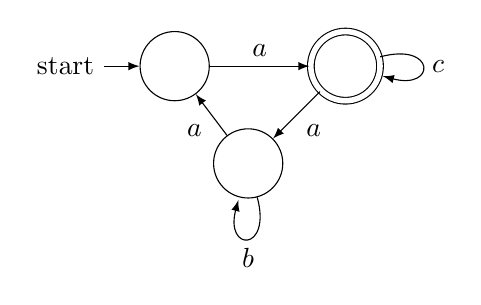
\begin{tikzpicture}[baseline=-2pc]
  \node [state,initial] (A) {};
  \node [state,right=3pc of A,accepting] (B) {};
  \node [state,below left=2pc of B] (C) {};
  \path [->] (A) edge node [above] {$a$} (B);
  \path [->] (B) edge [loop right] node [right] {$c$} ();
  \path [->] (C) edge [loop below] node [below] {$b$} ();
  \path [->] (B) edge node [below right] {$a$} (C);
  \path [->] (C) edge node [below left] {$a$} (A);
\end{tikzpicture}
\hfill
\ifkey{\color{red} $a(c|ab^*aa)^*$}\fi

\vspace{1pc}

\item (2 pts) Write the \textbf{simplest equivalent} regular expression for
  the following NFA.

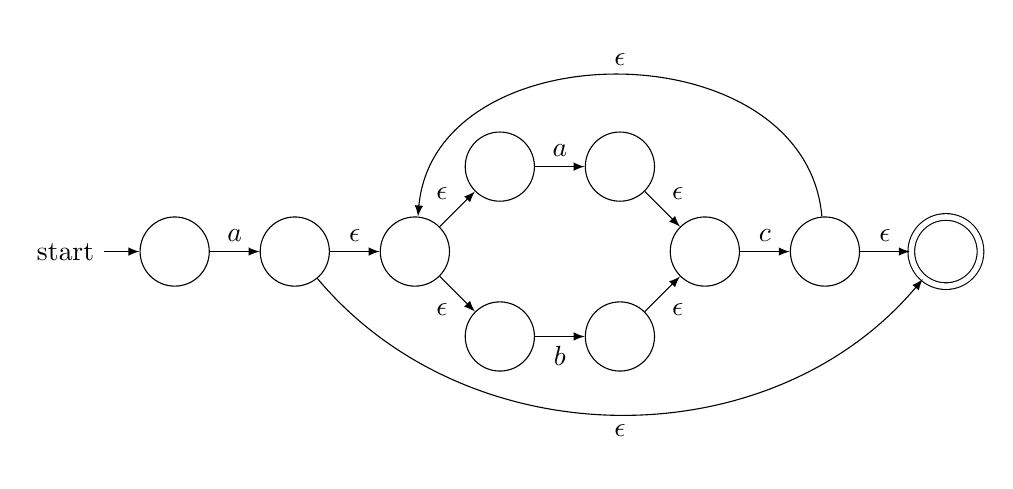
\begin{tikzpicture}[node distance=1.5pc,baseline=0pc]
    \node [state,initial] (00) {};
    \node [state,right=of 00] (0) {};
    \node [state,right=of 0] (1) {};
    \node [state,above right=of 1] (2) {};
    \node [state,right=of 2] (3) {};
    \node [state,below right=of 1] (4) {};
    \node [state,right=of 4] (5) {};
    \node [state,below right=of 3] (6) {};
    \node [state,right=of 6] (7) {};
    \node [state,right=of 7,accepting] (8) {};
    \path [->] (00) edge node [above] {$a$} (0)
               (2) edge node [above] {$a$} (3)
               (4) edge node [below] {$b$} (5)            
               (6) edge node [above] {$c$} (7)
    ;
    \choice 1 2 4 3 5 6
    \kleene 0 1 7 8
\end{tikzpicture}
\hfill
\ifkey{\color{red} $a\,((a\,|\,b)\,c)^*$}\fi

\end{enumerate}

\begin{problem}{10}{Grammars}
Write an \textbf{unambiguous grammar} that accepts the same language
as the grammar below, whose terminals are ``$\bigtriangleup$,''
``$\bigcirc$,'' and ``$a$.''  Make it so ``$\bigtriangleup$''
\textbf{associates left-to-right}, ``$\bigcirc$'' \textbf{associates
  right-to-left}, and ``$\bigtriangleup$'' is at a \textbf{higher
  level of precedence} than ``$\bigcirc$''.  E.g., so that
``$a\bigtriangleup a\bigtriangleup a \bigcirc a \bigcirc a$'' has a
unique rightmost derivation grouped like ``$(a\bigtriangleup
a)\bigtriangleup \big(a \bigcirc (a \bigcirc a)\big)$''

\[
\begin{array}{l}
E \rightarrow E\ \bigtriangleup\ E \\
E \rightarrow E\ \bigcirc\ E \\
E \rightarrow a
\end{array}
\]

\vbox to 8pc{
\ifkey{\color{red}
\[
\begin{array}{l}
E \rightarrow T\ \bigcirc\ E \\
E \rightarrow T \\
T \rightarrow T \ \bigtriangleup\ c \\
T \rightarrow a \\
\end{array}
\]
}\fi
\vfill
}
\end{problem}

\end{problem}

\newpage
\begin{problem}{25}{The SLR Parse Table}

Consider the grammar  \hspace{2pc}  \begin{tabular}[t]{>{\footnotesize}l>{$}l<{$}@{\ $\rightarrow$\ }>{$}l<{$}}
0: & X' & X \\
1: & X & b \\
2: & X & Y \\
3: & X & a X \\
4: & Y & b \\
\end{tabular}
\hspace{2pc}
\begin{minipage}[t]{16pc}
This generates strings of the form $a^*b$, e.g., $b$, $aaab$.  Here is
a derivation for the string $ab$ with the handles underlined:  $X'
\rightarrow \underline{X} \rightarrow \underline{a X} \rightarrow a
\underline{b}$.
\end{minipage}

\begin{enumerate}

\item (4 pts.) Show \textbf{two rightmost derivations} for $aab$
  and \textbf{underline the handles}.

\vbox to 4pc{
\ifkey\color{red}
$X' \rightarrow \underline{X} \rightarrow \underline{a X} \rightarrow a \underline{a X} \rightarrow a a \underline{b}$

$X' \rightarrow \underline{X} \rightarrow \underline{a X} \rightarrow a \underline{a X} \rightarrow a a \underline{Y}
\rightarrow a a \underline{b}$
\fi
\vfill
}

\item (4 pts.) Is this grammar ambiguous?  Why or why not?

\vbox to 3pc{

\ifkey
\color{red}Yes: there are two rightmost derivations for the same string.
\fi
\vfill
}

\item (4 pts.) Compute the following sets.  \textbf{Explain your reasoning.}

$\textsc{follow}(X) = \Bigg\{ \ifkey \textcolor{red} {\$} \fi \hspace{8pc} \Bigg\}$  \ifkey \quad \textcolor{red}{$X' \rightarrow X$ implies \$; $X \rightarrow a X$ gives nothing more} \fi

$\textsc{follow}(Y) = \Bigg\{ \ifkey \textcolor{red} {\$} \fi \hspace{8pc} \Bigg\}$ \ifkey \quad \textcolor{red}{$X \rightarrow Y$ implies \$; nothing further} \fi

\item (13 pts.)  Complete the \textbf{LR(0) automaton} and
  \textbf{SLR parse table} for this grammar. Mark all accepting states. \textbf{Indicate where
    the reduce/reduce error occurs.} 

\newcommand{\itemtab}[1]{
  \begin{tabular}{>{$}l<{$}@{\ $\rightarrow$\ }>{$}l<{$}} #1 
  \end{tabular}}

\vspace{2pc}

\ifkey
  \def\accepting{accepting}
\else
  \def\accepting{}
\fi


\begin{tikzpicture}[baseline=0pc]
\node [draw,minimum height=7pc,text width=8pc] (S0) {S0: 
  \itemtab{
    X' & \cdot X \\
    X & \cdot b \\
    X & \cdot Y \\
    X & \cdot a X \\
    Y & \cdot b}
  };

\node [draw,above right=of S0,minimum height=7pc,text width=8pc,\accepting] (S1) {
  S1: \ifkey\color{red}\itemtab{
    X & b \cdot \\
    Y & b \cdot}\fi
  };

\node [draw,right=of S0,minimum height=7pc, text width=8pc] (S2) {
  S2:
  \ifkey\color{red}\itemtab{
    X & a \cdot X \\
    X & \cdot b \\
    X & \cdot Y \\
    X & \cdot a X \\
    Y & \cdot b}\fi
  };

\node [draw,below=of S0,minimum height=7pc, text width=8pc, \accepting] (S3) {
  S3:
  \ifkey\color{red}\itemtab{
    X & Y \cdot}\fi
  };

\node [draw,below=of S2,minimum height=7pc, text width=8pc, \accepting] (S4) {
  S4:
  \ifkey\color{red}\itemtab{
    X & a X \cdot}\fi
  };


\node [draw,above=of S0,minimum height=7pc, text width=8pc, \accepting] (S5) {
  S5:
  \ifkey\color{red}\itemtab{
    X' & X \cdot}\fi
  };

\path [->] (S0) edge node [above left] {$b$} (S1)
                edge node [above] {$a$} (S2)
                edge node [right] {$Y$} (S3)
                edge node [right] {$X$} (S5);
\ifkey
\path [->,color=red]
           (S2) edge [out=5,in=-5,loop] node [right] {$a$} ()
                edge node [above] {$Y$} (S3)
                edge node [right] {$X$} (S4)
                edge node [right] {$b$} (S1);
\fi
\end{tikzpicture}
\hspace{3pc}
\setlength{\tabcolsep}{10pt}
\renewcommand{\arraystretch}{3}
\begin{tabular}{r|ccc|cc}
 & a & b & \$ & X & Y \\
\hline
0 & s2 & s1 & & 5 & 3 \\
1 & & &\ifkey\color{red} r1/4\fi & & \\
2 & \ifkey\color{red} s2\fi & \ifkey\color{red} s1\fi & & \ifkey\color{red} 4\fi & \ifkey\color{red} 3\fi\\
3 & & & \ifkey\color{red} r2\fi& & \\
4 & & & \ifkey\color{red} r3\fi& \\
5 & & & \ifkey\color{red} \Checkmark\fi& & \\
\end{tabular}

\vfill

\end{enumerate}

\end{problem}

\newpage

\if 0
http://jsmachines.sourceforge.net/machines/slr.html

E' -> E
E -> E * T
E -> T
T -> T + id
T -> id

1	0		id + id * id $	s3	
2	0 id 3		+ id * id $	r4
3	0 T		+ id * id $	2
4	0 T 2		+ id * id $	s5
5	0 T 2 + 5	id * id $	s7
6	0 T 2 + 5 	id 7	* id $	r3
7	0 T		* id $		2
8	0 T 2		* id $		r2
9	0 E		* id $		1
10	0 E 1		* id $		s4
11	0 E 1 * 4	id $		s3
12	0 E 1 * 4 id 3	$		r4
13	0 E 1 * 4 T	$		6
14	0 E 1 * 4 T 6	$		r1
15	0 E		$		1
16	0 E 1		$		acc

\fi

\begin{problem}{20}{Rightmost Derivations, Bottom-Up Parsing}

For the following grammar with terminals $\times$, $+$, and
\textbf{n} and non-terminals $T$ and $E$

\[
\begin{array}{rl}
1: & E \rightarrow E\ \times\ T \\
2: & E \rightarrow T \\
3: & T \rightarrow T\ +\ \textbf{n} \\
4: & T \rightarrow \textbf{n} \\
\end{array}
\]

\begin{enumerate}

\item (5pt) Give a \textbf{rightmost derivation} for ``\textbf{$n + n \times n$}'' and
  \textbf{underline the handles}.

\vbox to 8pc{
\ifkey{\color{red}
$
E
\rightarrow \underline{E \times T}
\rightarrow E \times \underline{n}
\rightarrow \underline{T} \times n
\rightarrow \underline{T + n} \times n
\rightarrow \underline{n} + n \times n
$
}
\fi
\vfill
}

\item (15 pts.) \textbf{Show the steps} a shift-reduce parser would
  take on such an input.  I've started the table for you.

\vspace{1pc}

\vbox to 20pc{
\begin{tabular}{@{\hspace{5pc}}rl@{\hspace{5pc}}l}
\toprule
\textbf{Stack} & \textbf{Input} & \textbf{Action} \\
\midrule
 & n + n $\times$ n \$ & Shift \\
\ifkey
\color{red}n &\color{red} + n $\times$ n \$ &\color{red} Reduce 4 \\
\color{red}T &\color{red} + n $\times$ n \$ &\color{red} Shift \\
\color{red}T + &\color{red} n $\times$ n \$ &\color{red} Shift \\
\color{red}T + n &\color{red} $\times$ n \$ &\color{red} Reduce 3 \\
\color{red}T     &\color{red} $\times$ n \$ &\color{red} Reduce 2 \\
\color{red}E     &\color{red} $\times$ n \$ &\color{red} Shift \\
\color{red}E $\times$     &\color{red} n \$ &\color{red} Shift \\
\color{red}E $\times$ n     &\color{red} \$ &\color{red} Reduce 4 \\
\color{red}E $\times$ T     &\color{red} \$ &\color{red} Reduce 1 \\
\color{red}E                &\color{red} \$ &\color{red} Accept \\
\fi
\end{tabular}
\vfill
}


\end{enumerate}

\end{problem}




\end{document}

% Local Variables:
% compile-command: "make midterm.pdf"
% End:
